\documentclass{article}
\usepackage[utf8]{inputenc}


\usepackage{titlesec}
\usepackage{rotating}
\usepackage{easylist}
\usepackage{amssymb}
\usepackage{natbib}
\usepackage{graphicx}
\usepackage{url}
\usepackage{textcomp}
\usepackage[T1]{fontenc}

    % By default the URLs are put in typewriter type in the body and the
    % bibliography of the document when using the \url command.  If you are
    % using many long URLs you may want to uncommennt the next line so they
    % are typeset a little smaller.
    % \renewcommand{\UrlFont}{\small\tt}
    
\setcounter{secnumdepth}{4}

\titleformat{\paragraph}
{\normalfont\normalsize\bfseries}{\theparagraph}{1em}{}
\titlespacing*{\paragraph}
{0pt}{3.25ex plus 1ex minus .2ex}{1.5ex plus .2ex}

\usepackage[margin=0.8in]{geometry}

\begin{document}

\begin{titlepage}
                % \newgeometry{top=25mm,bottom=25mm,left=38mm,right=32mm}
                \setlength{\parindent}{0pt}
                \setlength{\parskip}{0pt}
                % \fontfamily{phv}\selectfont

                {
                                \Large
                                \raggedright
                                Imperial College London\\[17pt]
                                Department of Electrical and Electronic Engineering\\[17pt]
                                Final Year Project Report 2015\\[17pt]
 
                }

                \rule{\columnwidth}{3pt}
                \vfill
                \centering
                  %\includegraphics[width=0.7\columnwidth,height=60mm,keepaspectratio]{background/iCub_model.jpg}
                \vfill
                \setlength{\tabcolsep}{0pt}

                \begin{tabular}{p{40mm}p{\dimexpr\columnwidth-40mm}}
                                Project Title: & \textbf{Cloud Robotics Infrastructure} \\[12pt]
                                Student: & \textbf{Yuchen Wang} \\[12pt]
                                CID: & \textbf{00597191} \\[12pt]
                                Course: & \textbf{EIE4} \\[12pt]
                                Project Supervisor: & \textbf{Dr Jeremy V. Pitt} \\[12pt]
                                Second Marker: & \textbf{Dr Javier A. Barria} \\
                \end{tabular}
\end{titlepage}




% \title{Simulator for Decentralised Community Energy Systems \\ Final Year Project Report}

% \author{Yuchen Wang}
% \date{8th June 2015}

% \maketitle  %Title Page

\clearpage  %New page for abstract
\begin{abstract}
In many developing countries the electricity grid network is underdeveloped, causing low levels of rural electrification. However, electricity access in these rural communities are not non-existent. There are a number isolated and independent electricity generators owned by individuals, NGOs and local government institutions. This project explores the feasibility of a Decentralised Community Energy System which utilises these isolated sources of electricity to create a community micro grid. It is planned to conduct the feasibility study with the help of a simulation to be developed using Presage2 and Java. This report outlines the deliverables, planning process, background research, and the design and implementation of the simulation model. 

%TODO: Complete this once report is finished.
\end{abstract}
\clearpage

\tableofcontents
\clearpage

\section{Introduction and Background}
In many areas of rural developing countries, there are often no wide-spread access to a continuous and reliable electricity supply such provided by the country's electricity grid \cite{IEA-web:2015}. However there exists many isolated sources of electricity generation such as solar panels and standalone diesel generators utilised by relatively wealthy households, shops and buildings belonging to large organisations. 

The aim of this project is to explore the idea of using a holonic institution to model a Decentralised Community Energy System which bring together the existing decentralised generation infrastructure to provide an affordable source of reliable electricity for users in rural communities. 

Over the course of this project, a multi-agent simulation model was built using Presage2 with individual households and businesses modelled agents. The agents can be grouped together to form communities such as villages, which in turn can be grouped together to form a larger entity such as a district or a province. 

%To do: cite here:
With humans being social creatures who are likely to band together to form communities, the structure of the decentralised energy system model will be designed in a similar way with holonics. The structure of how the simulation is designed is based on the design of holonic systems \ignore{\#\# CITE JP paper HERE \#\#}. In the case of this project, the simulation will be to distribute fairly electrical power between interrelated agents which are in turn composed of interrelated subagents recursively, until reaching lowest level of subagents (households and businesses). 

To allow the model to be realistic, candidate rural communities with no access to a source of reliable electricity will be identified using data and research. Additional data on usage habits and potential generation profiles of generators in the candidate areas will be obtained through research to produce a simulation model that is accurate and relevant.

Include:
\begin{itemize}
\item Design Choices: Holonics, design of objectives
\item difficulties and how they were designed:
\subitem Out of order parallel execution
\subitem Presage
\subitem One action per time step
\item Discovery or invetion of something novel?
\item What did you learn:
\subitem Java, Presage, Software design
\end{itemize}


This report outlines the design, implementation and testing of a holonic multiagent simulation of a decentralised energy system. 

\section{Background}

\subsection{Electricity as a Common Pool Resource}
A Common Pool Resource is a depletable resource which can be utilised by a group of people, characterised by a reduction in the availability of this resource as individuals withdraw or utilise this resource \cite{Ostrom:90}.  Electricity can be a Common Pool Resource if there exists a finite amount of electricity generation capacity. As users connect demand appliances to the generators, the availability of electricity supply for additional demand diminishes.

In developing communities with significant generation from renewable sources such as wind and solar, the availability of power is subject to variation between periods in time. This inherent volatility in the amount of available resource could increase the likelihood of selfish actions of by individuals in the community.

Common Property Regimes can be formed to maintain the Common Pool Resources by controlling the access to the resource. Over the course of the project, various means of controlling access to electricity will be explored. 

\subsection{Decentralised Community Energy Systems as a Holonic System}
A holonic system (or holarchy) is a system which is composed of interrelated subsystems or institution, each of which are in turn composed of sub-subsystems  or institution and so on, recursively until reaching a lowest level of "elementary" subsystems. Each system, sub system or institution has a well-defined set of goals or objectives which is achieved through enforcing a set of rules on its members (subsystems, sub-institutions and elementary entities). \ignore{cite Pitt}

In the case of the Decentralised Community Energy system model, the holonic system would be composed of communities which are composed of sub-communities recursively until reaching the lowest level of "elementary" subsystem which would be households in this case. Each community or institution has the goal of fairly allocating electricity to all members. This goal would be achieved with the assumption that they are provided with the necessary infrastructure and powers for enforcing quotas and contribute to a common pool of electricity.


\subsection{Rural Communities in Rwanda}
With an estimated 25\% rural electrification rate in 2009 \cite{IEA-web:2015}, rural Africa is one obvious candidate for simulation scenarios. Vast amounts of rural communities remain un-electrified. For a realistic simulation scenario, knowledge of existing infrastructure in place will need to be obtained. With many areas within many countries in Africa, Rwanda in particular has been identified as a good potential simulation scenario to research. Data is difficult to source for rural communities in developing countries, however in the case of Rwanda, some data can be easily from the student society e.quinox. e.quinox is a student-led society which aims to find a scalable solution for rural electrification who mainly operate in Rwanda \cite{e.quinox-web:2015}. The subsections below outline some of the ways remote rural communities are able to access electricity in Rwanda.

\subsubsection{Electricity Generation}
One of the solutions currently being implemented by e.quinox is the "Energy Kisok" model \cite{e.quinox-EK-web:2015}. The "Energy Kiosk" model features an Energy Kiosk - a building where the generation, storage and distribution of electricity takes place.
In e.quinox operated kiosks, electricity is generated from renewable sources.
Traditionally, this has been with solar panels. However, hydro-electric generation has been demonstrated to be feasible with the recent construction of a "Hydro Kiosk" at Rugaragara Falls in Southern Rwanda.

\subsubsection{Storage and Distribution}
Within each kiosk, electricity that is generated is stored in storage batteries placed in the kiosks. The storage batteries regulate power output and allows access to electricity in the kiosk even during periods of no electricity generation.

\paragraph{Battery Box}
In the absence of any electricity distribution infrastructure, e.quinox has traditionally provided a number of portable batteries for the purpose of electricity distribution. An example of the portable batteries can be seen in Figure \ref{fig:AmaziBox}.

\begin{figure}[h!]
\centering
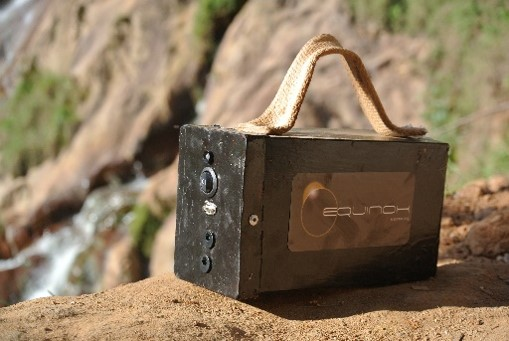
\includegraphics[scale=0.7]{Images/AmaziBox.jpg}
\caption{First Generation e.quinox Battery Boxes deployed at Rugaragara Falls Kiosk}
\label{fig:AmaziBox}
\end{figure}

Consumers from local community pay to hire the battery boxes under one of two payment schemes: pay-per-recharge and pay-per-month \cite{e.quinox-Hydro-web:2012}. The biggest difference between the two schemes are that users can recharge as often as they would like with pay-per-month. Both payment schemes involve the recharge of the boxes at the energy kiosk when they are depleted of energy.

A potential use case of this project can be the simulation of charging of battery boxes at an energy kiosk. This could alleviate congestion and improve asset utilisation of the existing distribution systems by reducing the turn-around time of battery boxes for customers.

\paragraph{Micro Grid}
With the recent completion of a hydro-electric kiosk. e.quinox for the first time has a kiosk with access to an always-on generator. With a limited number of battery boxes in circulation and a constant generation available during the off-peak hours, there is excess capacity for electricity generation.

To improve utilisation of the generator in the kiosk, e.quinox has recently started conducting a feasibility study into constructing a transmission line and a distribution network which will serve a village near the kiosk with a view to make the most of the electricity generated.

Preliminary surveys conducted in the nearest village to the kiosk indicates the demand could exceed the amount of excess power generated by the kiosk. 

The result of this project can be used in conjunction with e.quinox to conduct the feasibility study of implementing the Micro-Grid. Should a trading platform for energy also be built, the Micro-Grid could serve as a test-bed for this new system.

\paragraph{Standalone Solution}
The Standalone Solution is an independent electrification solution which was recently developed by e.quinox for customers who live far from energy kiosks.

The Stand-alone solution consists of a pay-as-you-go solar electricity generation and storage kit, known as the Izuba.Box \cite{e.quinox-Standalone-web:2012}.  With the Izuba.Box, customers no longer have to travel regularly back to the Energy Kiosk for electricity. Solar panels are installed on the customer’s roof, and is connected to a sealed box which contains a large battery box. The attached large battery box allows a regulated power output and access to electricity during dark hours. 

With the customers not returning to Energy Kiosks, the battery boxes are not hired out like the battery boxes are. The high capital costs of the independent solar system is spread over typically a two year rent-to-own payment plan using a mobile payment system.

It is hoped that the Standalone Solution and additional generation from the Energy Kiosk can be complemented the battery boxes in circulation to provide a continuous access to electricity to all households in the village.

\Paragraph{In context of the simulation}
In developing countries such as Rwanda, poor communities with no access to grid electricity are often in isolated locations. In these areas, fuel for generators are often difficult to obtain. Other available sources of electricity such as solar and wind power are highly dependent other variables such as weather. It is also highly unlikely that they will have access to redundancies to ensure continual access much like the electricity we receive from the national distribution and transmission network in the UK. It is therefore beneficial for systems such as the one we are modelling as it has lower barriers to entry than access to 

\begin{figure}[h!]
\centering
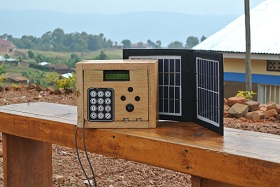
\includegraphics[scale=3]{Images/standalone_box.jpg}
\caption{First Generation Izuba.Box deplyed in Minazi, Northern Rwanda}
\label{fig:IzubaBox}
\end{figure}

% \subsection{Additional Research}
% e.quinox in Rwanda only presents us with one scenario. Additional research is required for other regions such as South America and the Indian Subcontinent to look at potential new scenarios and use cases for various generators and electrical appliances.

% The information above only outlines the existing infrastructures in place. Additional work needs to be done to obtain relevant usage data from e.quinox customers and other electricity users to accurately build a relevant generation mix and demand model.

% In some regions such as Minazi, e.quinox provides the only source of accessible electricity for the local populace. Data on their usage should be more readily available than some of the other locations in other countries. 

\section{Requirements}


It is therefore required that the simulation platform will have the following features:
\begin{itemize}
  \item Multiple Forms of Generation: Renewable and Non-renewable generators which can operate continuously or discontinuously
  \item Realistic Generator Models: Programmable variable generation power output to simulate wind and solar power
  \item Multiple demand centres: the simulation will be of one or more communities operating with a number of households/businesses requiring electricity
  \item Self organising by the system to appropriate the available power fairly to all users
\end{itemize}

As this is a simulation to be implemented in Presage2, there are no specific requirements which must be adhered to with regards to speed, portability and performance.  

The simulation is to be developed using Presage2. It is hoped that a network of Decentralised Community Energy Systems can be simulated, and a working trading system can also be developed for the trading of limited available energy within communities towards the end of the project time frame. 


\section{Project Planning}
Following a number of supervisor meetings with Dr Pitt, a number of work items have been identified. A Gantt Chart was created to facilitate the planning and tracking of the project progress. A copy of the current Gantt Chart can be seen in Figure \ref{fig:GanttChart}. The Gantt Chart was a continuous working document which will be update as the project progresses. Tasks were added as new ideas for the project became available. 

\begin{figure}[h!]
\centering
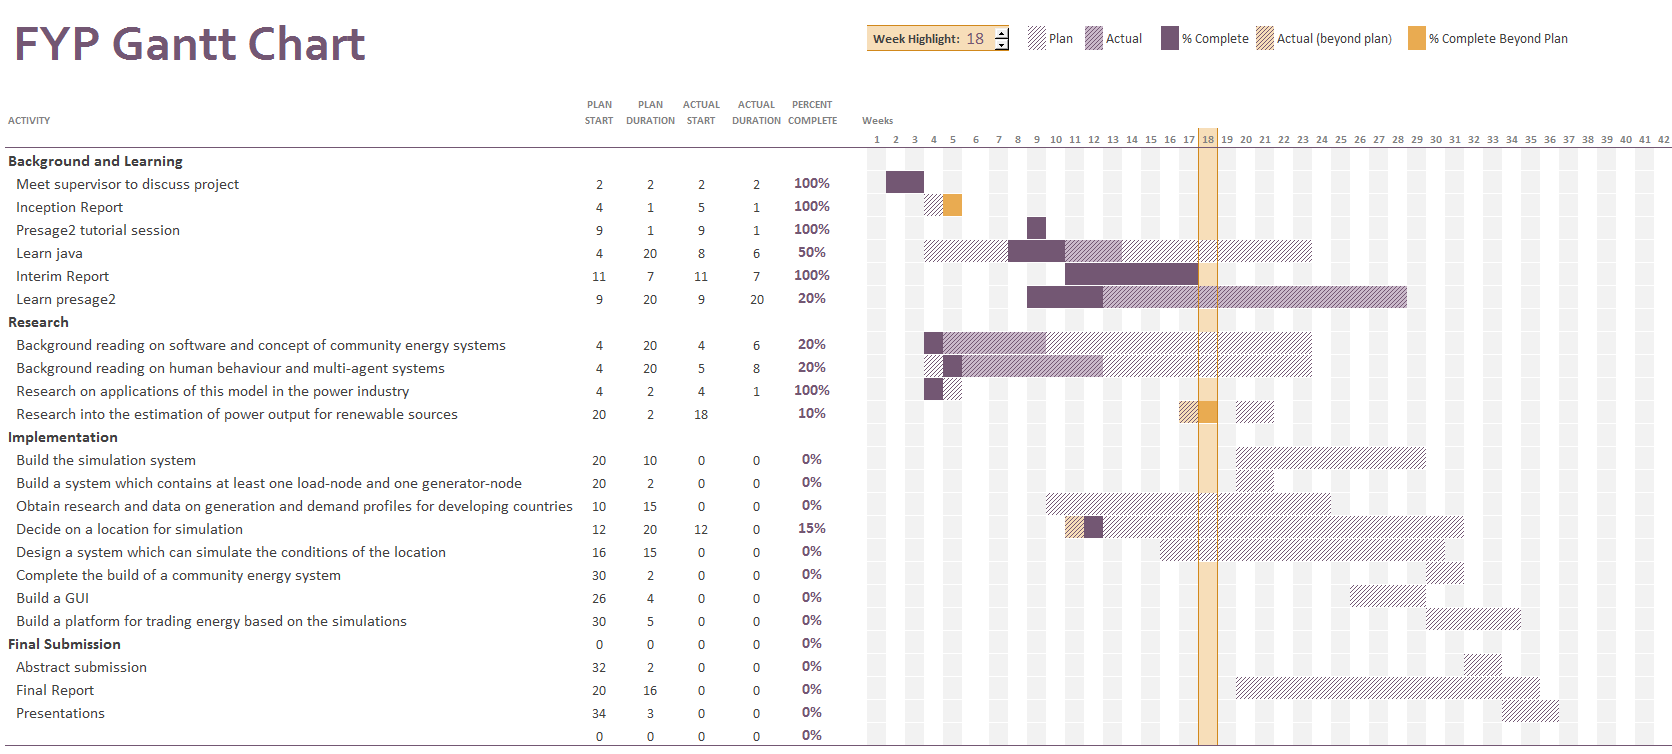
\includegraphics[scale=0.5, angle=90]{Images/GanttChart.png}
\caption{Up to date Gantt chart}
\label{fig:GanttChart}
\end{figure}

\clearpage

\section{Implementing with Presage2}
\subsection{About Presage2}
PRESAGE2 is a simulation platform for multi-nodal or Agent simulation of societies. The platform was built and is currently maintained by PhD students within Imperial. This platform enables the project to investigate the impact of agent design (such as household behaviour), network properties (constraints on access) and the physical environment on individual agent behaviour and long-term global network performance \cite{Presage2-Desc:2015}. In the case of this project, each Node/Agent can represent individuals, households, businesses or generators. 

\subsection{Implementing the Micro Grid in Presage2}
Using Presage2, a network akin to the simplified model in Figure \ref{fig:SimpleModel} will be created and simulated. The Agents are reprsented by the Circles labeled A-H, and the various demand/generation equipment connected on the outside of the network represent the properties the Agents are expected to have.

\begin{figure}[h!]
\centering
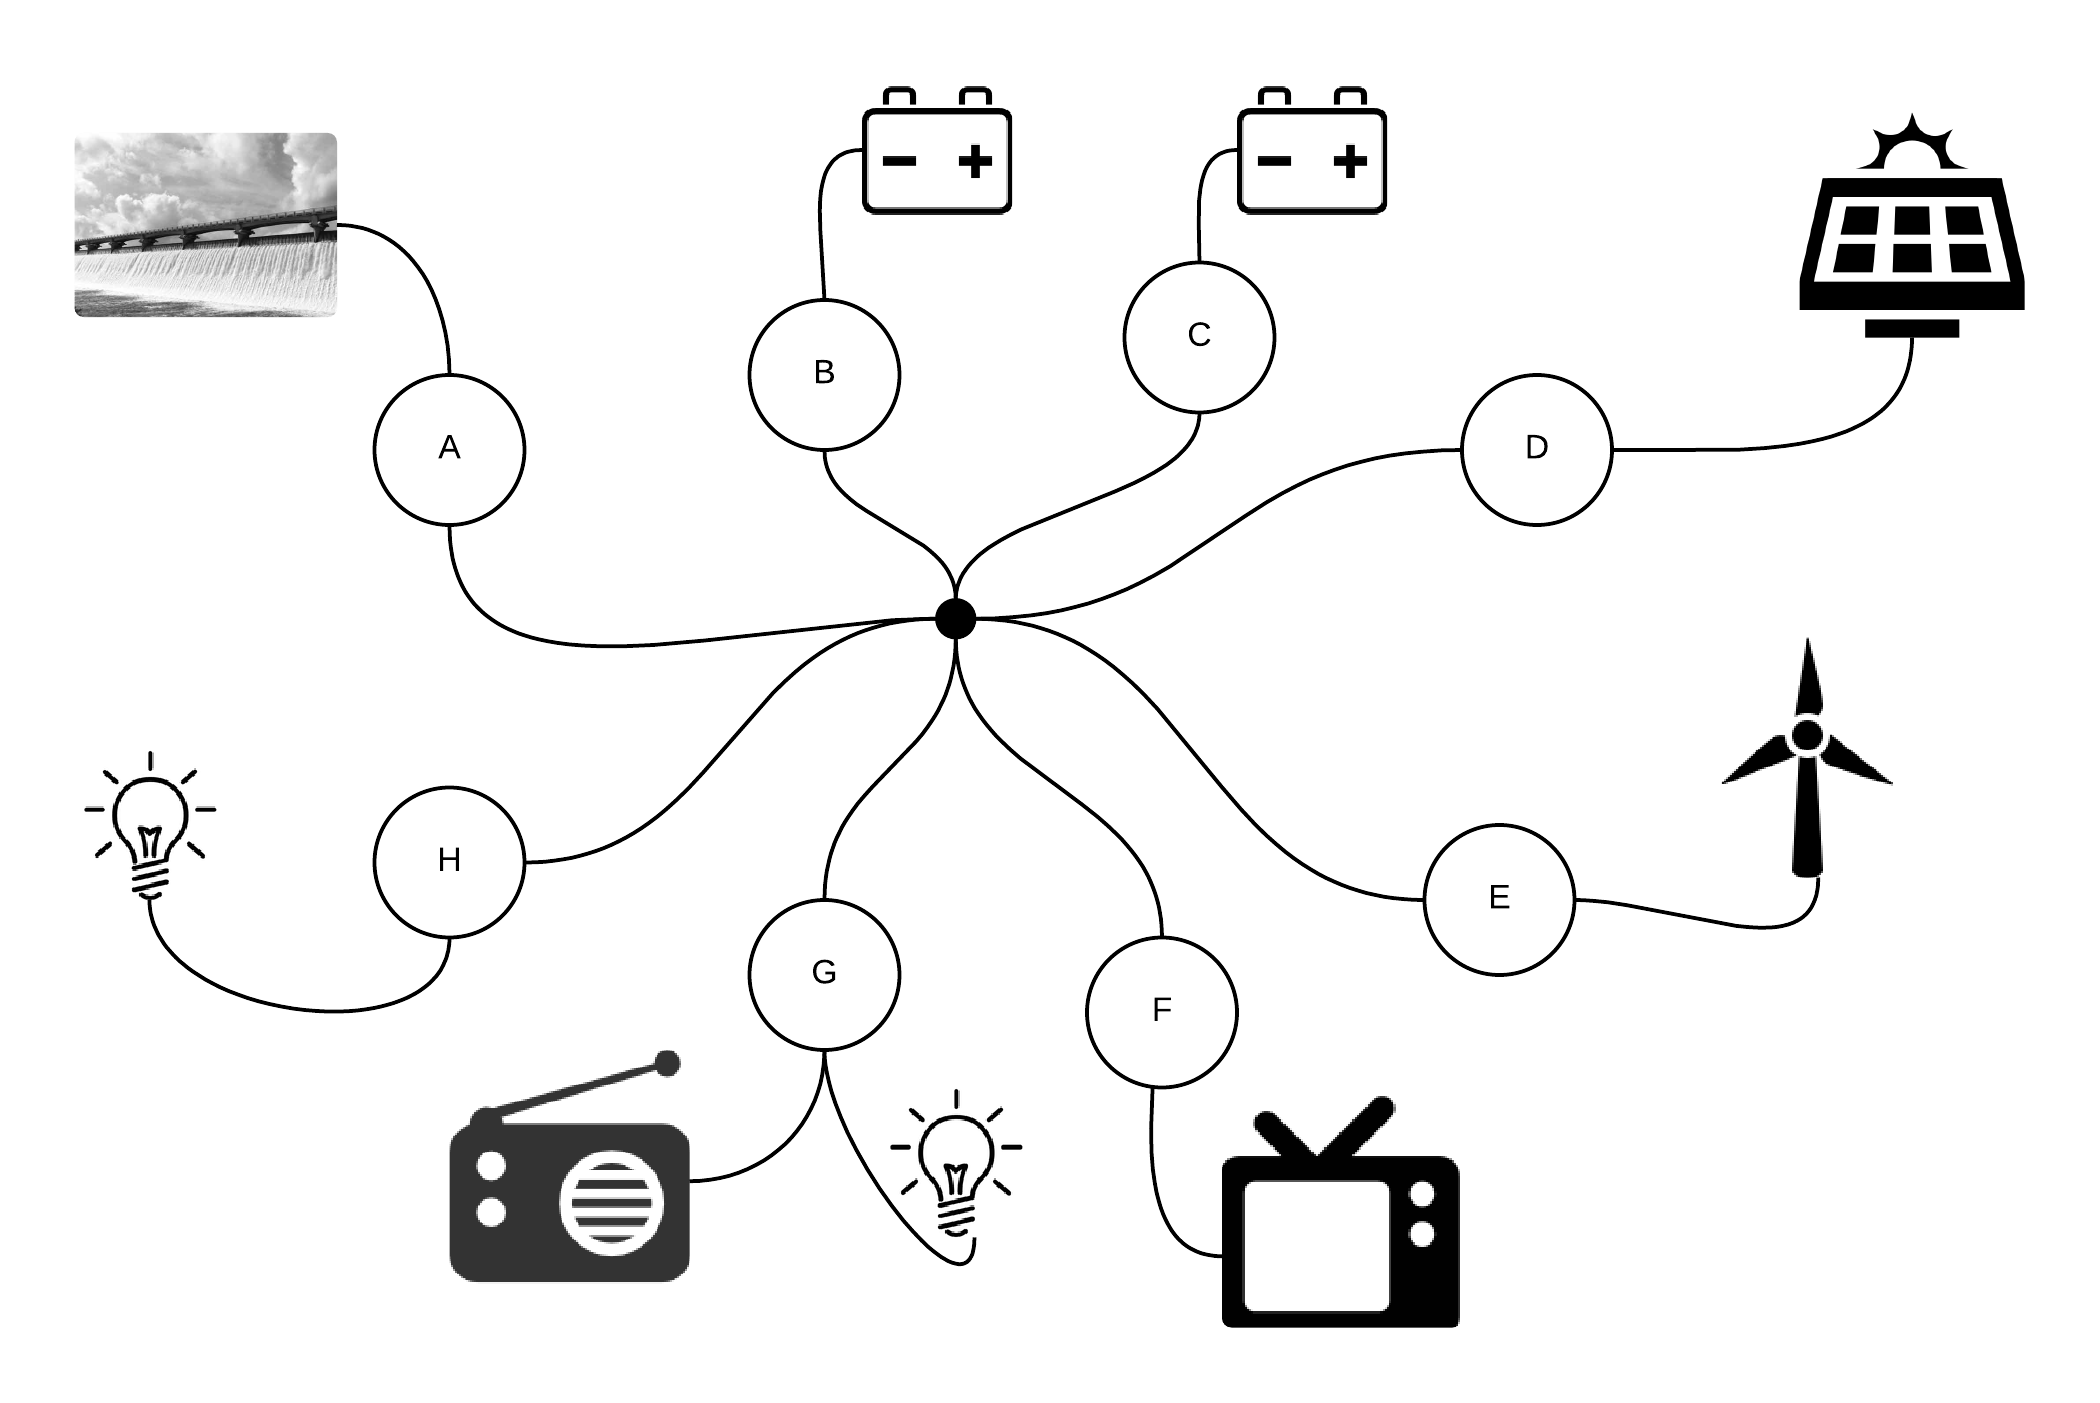
\includegraphics[scale=0.8]{Images/Model.png}
\caption{A simplified model diagram}
\label{fig:SimpleModel}
\end{figure}

In the immediate future, it is hoped that this tool could be used to aid the feasibility study of the Micro-Grid to be implemented in Rugaragara Falls. Should there be time, an energy trading platform will be designed and built based on the model created in this project to provide adequate electricity access to all members of the community. However, the energy trading platform would require a different design and implementation scheme which is not included in this report.

The sections below outlines the various properties each Agent must be able to take and how they could be implemented for the simulation scenario of rural communities in Rwanda. All of the properties must be allowed to exist on the same Agent during simulation.

\subsubsection{Agent Properties}

\paragraph{Generator}
Generators will be assumed to be generating power, and not draw any power from the Micro Grid. Four types of generator properties will be implemented in this simulation model: 

\begin{itemize}
  \item Hydro-electric - a constant source of energy based on a mixture of historical data and projections.
  \item Solar - a source of energy following the typical output profile of a solar panel connected to households.
  \item Wind - a source of energy which will be highly variable in output.
  \item Diesel - a constant source of energy.
\end{itemize}

With the power output of renewable sources of energy such as wind and solar being non-predictable in nature, one of two approach will need to be undertaken to model these sources:
\begin{itemize}
  \item A probabilistic generating factor is applied to the generators. This is a constant amount of power each solar panel or wind turbine is assumed to produce during some hours of the day that is to be determined. 
  
  \begin{itemize}
    \item * If this method is to be used, the model needs to be implemented in such a way to allow dynamic load-shedding and load-dumping.  
  \end{itemize}
  
  \item A probabilistic generation power output curve based on the least sunny / least windy days
  \begin{itemize}
    \item * If this method is to be used, sufficient weather and generation data will need to be obtained to implement this method
  \end{itemize}
\end{itemize}

More research will need to be conducted to look at which of the two methods will be more suitable in this application. Both methods are in use by distribution networks in the UK for assessing network congestion \cite{IPSA-web-constraint:2015}.

\paragraph{Demand}
The Demand property will only use electricity in the system. These represent households and businesses in the nearby village. Assumed demand curves will be produced from survey data of potential customers in the area for the initial testing. Should the survey data not be available for the area, a reasonable approximation will be made based a predicted usage habits of the wider local population.

It is anticipated that the final simulation will have a desired demand profile that each Demand-based agent will aim for by trading its allocated energy with other agents. However, the change in demand profile due to trading of energy must be able to satisfy the expected behavioral habits of the local inhabitants. These habits should include restrictions such as no trading during hours of sleep for households. What the habits will be, and how this will be implemented will be determined after some additional research into the area.

\paragraph{Storage}
The Storage property is a dynamic entity which can act as a generator or demand depending on the network utilisation and available power. These storage devices will be batteries of various types that will be connected to the network.

Storage properties will be attached to households which own battery boxes. The Storage property must have the capability to prioritise the allocation of its stored energy for certain Agents. For example, the energy output of Storage-only agents could be made to always prioritise the households they are attached to. If the battery box is communal or belongs to a centralised entity such as an e.quinox Energy Kiosk, then no priority will be attached.

\section{Simulation of the Micro Grid with Presage2}
With the village to be electrified implemented as a model with Presage2, studies will be conducted to determine the best allocation of resources to keep the customers in the village in a reasonably happy state. This would entail that every Agent will be able to consume all of its required energy consumption in the simulation period with a consumption/demand profile which follows all of the properties defined in the Demand property.

Further studies will also be conducted to determine the effects of varying the number of various properties in the network to create for example, a demand-heavy network or a generation-heavy network.  

\subsection{Model Assumptions}
With the Micro Grid model running under Normal Operation, a number of assumptions will be made to simplify the implementation of the model:
\begin{itemize}
\item No losses will be incurred by cables
\item All load on the network will be resistive
\item Only basic appliances such as phones, lights and fridges will be connected to the vast majority of households. A communal fridge-freezer and TV will be available at one of the households
\item Simulations will be run over a variable 1-7 day period
\end{itemize}

\section{Further work}
To facilitate the completion of this project, research will need to be carried out in the following areas:
\begin{itemize}
\item Continual updating of the Gantt Chart to track progress.
\item Research into additional sources of demand and load in rural developing countries and their typical usage to produce suitable realistic generation/demand curves for the simulation.
\item Consumer behaviour of the local population to determine a suitable demand curve, and the properties which are required to be part of the Demand property. e.quinox recently conducted a survey trip in January. The surveys will be used to produce potential demand profiles for the project.
\item Research into electricity generation and distribution infrastructure/equipment available in rural developing countries.
\item Number of households in the village will need to be determined to construct a realistic model.
\item The solar irradiation and photovoltaic cell generation profile for solar panels in developing countries will need to be reliably estimated. Preliminary research suggests an absence of data in this area. Data for Developed countries with similar climates could be used as an estimator.
\item Determine how to best estimate the output of a renewable source of energy dependent on the weather or time of day.
\item Typical storage sizes for battery storage units.
\item Design of Agents in Presage2 for the simulation.
\item Methods for implementing the simulation in Presage2.
\item A variety of rules and other management systems designed to efficiently allocate electricity access.
\end{itemize}

\subsection{Risks and Uncertainties}
\paragraph{Planning}
The simulation is to be built using Presage2 and Java. The biggest risk of any software project is under-estimating the time of completion, causing delays and ultimately an under-developed final product. To reduce to risks of time under-estimation, the Gantt chart will be employed and updated regularly. An action log of tasks and their time taken for completion will be kept and reviewed continuously to help further reduce to risk of under-estimating time completion of tasks. 

\paragraph{Data}
To produce realistic models with applicable results, relevant environmental and other technical data will need to be obtained over the course of this project. However, with underdeveloped data-collecting infrastructure in many developing countries, the obtaining of such information could prove difficult. To help gather this information, it may be necessary to use a combination of secondary sources such as e.quinox team members and data from other locations with established data-collecting infrastructure.

\section{Testing}
The final product of this project should be a realistic simulation of a Decentralised Community Energy System. To produce the simulation, each of the following features will be tested to ensure they work individually and together:

\begin{itemize}
\item A network of Agents able to trade electricity with each other.
\item Agents are able to utilise energy. The amount of energy utilised can be pre-determined manually by an operator of the simulation or automatically with an algorithm.
\item Agents are able to generate an amount of energy corresponding to a pre-allocated fixed output, or an amount based on their assigned Generation Profiles.
\item Each Agent is able to utilise and generate electricity at the same time.
\end{itemize}
%If data is available for the potential customers in Rugaragara, the simulation could be used in %conjunction with the feasibility study

\section{Extensions}
So far, the works carried out will be only be applicable for one community in rural Rwanda. It is hoped that work will be carried out to make this applicable to other communities by including more generation types such as biogas, and more types of appliances owned by each house.

In addition, the e.quinox Micro Grid is currently undergoing feasibility studies. If time allows, a system could be designed and built for the Micro Grid to allow the trading of electricity between households to guarantee electricity supply for when it is needed. This system however will have a completely different set of requirements, which will be drawn up after the completion of this project.

\section{Conclusion}
Since October, an attempt has been made on understanding the properties of Common Pool Resource, and how electricity can be a Common Pool Resource in the context of a Decentralised Community Energy System. An attempt will be made to build a simulation of a Decentralised Community Energy System which can utilise existing infrastructure in developing countries. 

The simulation of the Decentralised Community Energy System will be used to explore possible utilisation patterns within rural communities, and also explore controls for regulating the use of electricity. If the study proves to be successful, an attempt at designing and implementing a trading platform for Decentralised Community Energy Systems will be made. 
\bibliographystyle{plain}
\bibliography{references}

\end{document}
